%!TEX root = ../fbi.tex

\newcommand{\uL}{\mathbf{L_0}}
\newcommand{\bL}{\mathbf{\bar{L}_0}}

\section{Entanglement spectrum}
\label{sec:ES}

The quasi-1D cylinder geometry is convenient for calculating the
entanglement spectrum for entanglement cuts transverse to the long direction of the
cylinder. Here, the entanglement spectrum $\varepsilon_i$ is defined through the spectrum
$\rho_i$ of the reduced density matrices $\rho_{L/R}$ obtained for a bipartition of the state,
where we have $\varepsilon_i = -\log \rho_i$.
The corresponding eigenvectors of the reduced density matrices
are referred to as Schmidt states $\ket{\psi^{(i)}_{L/R}}$. 
The Schmidt decomposition 
\beq
\ket{\psi} = \sum\limits_i \sqrt{\rho_i}
\ket{\psi^{(i)}_{L}}\ket{\psi^{(i)}_{R}}
\label{eq:schmidt}
\eeq
relates the Schmidt states to the original wavefunction and is useful to keep in mind
when interpreting the entanglement spectrum.

To extract the entanglement spectrum exactly,
we use a method proposed in Ref.~\onlinecite{cirac2011}.
In the setup given here, the exact representation of the HFBI state as a PEPS of
fixed bond dimension implies an upper bound on the number of non-zero $\rho_i$; 
for the cut shown in Fig.~\ref{fig:FBI_PEPS_2}, this upper bound is $\chi=2^W$.

Upon computation of the entanglement spectrum, we find that this bound is saturated,
so that there are precisely $2^W$ contributing terms in Eq.~\ref{eq:schmidt}.
This fact can be simply understood without reference to the PEPS representation:
Each of the $w$ plaquettes on the cut can contribute its one boson either to the left
or the right of the cut, and this is the complete source of the uncertainty
of the state on one half of the cut when ignoring the state on the other half.

We can form a set of $2^W$ vectors $|\sigma_1,\ldots,\sigma_W)$ that correspond to the
choices for the auxiliary degrees of freedom of the PEPS across the cut. The PEPS defines
a map from these boundary vectors to physical states in the bulk of the
semi-infinite cylinder, which we denote as $\ket{\psi_L^{(\sigma_1, \ldots, \sigma_W)}}$;
on the subspace of physical states spanned by Schmidt states with non-vanishing contribution
to the reduced density matrix, this map is invertible and can be computed explicitly.

%We can construct a set of states $\ket{\psi_L^{(\sigma_1, \ldots, \sigma_W)}}$ that 
%correspond to the state on the left half of the cylinder when the $i^{th}$ plaquette
%contributes $\sigma_i \in {0, 1}$ bosons to the left half of the cylinder. 
%These states are not orthogonal, but they are linearly independent and span the same
%$2^W$-dimensional space as the Schmidt states $\ket{\psi^{(i)}_{L}}$.
%These states are precisely the states you would get by contracting the PEPS in
%Fig.~\ref{fig:FBI_PEPS_2} on the left half of the cylinder with fixed values
%$\sigma_i$ for the $W$ virtual bonds at the boundary.

Translation around the cylinder acts in the natural way on the states 
$\ket{\psi_L^{(\sigma_1, \ldots, \sigma_W)}}$ by permuting the values of 
$\sigma_i$, $\sigma_i \to \sigma_{i+1}$.
Although the boson number on the half-infinite cylinder is infinite, we can define for
each basis element a $U(1)$ charge corresponding to the number of bosons to the
left of the cut relative to a uniform background charge,
\begin{equation}
Q_L = \sum_i (\sigma_i - \frac12).
\end{equation}
Only relative charges between states will be important for our conclusions, and the precise
way in which background charge is accounted for does not matter.
Each state is paired with a corresponding state on the right half of the cylinder with opposite charge.

We can block-diagonalize the reduced density matrix
for a half-infinite cylinder in both the U(1) charge and transverse momentum
quantum numbers, allowing us to perform more efficient calculations. 
In addition, we can assign quantum numbers to both the Schmidt states and the entanglement
spectrum. This property is generically true for U(1) symmetric and translationally invariant PEPS
on a cylinder, although not in general true for arbitrary symmetry groups.
This point is elaborated on in Appendix~\ref{Appendix:MPS}.

% This seems overly complicated.
%As shown in \cite{perezgarcia2008}, a translationally invariant MPS can be
%assigned a projective representation of the on-site symmetry group, acting on
%the virtual legs, that maps Schmidt states to degenerate Schmidt states.
%For the MPS formed by the HFBI, we find that the U(1) boson number symmetry
%and the$\mathbb{Z}_L$ translational symmetry around the cylinder circumference
%are represented linearly. Each Schmidt state can thus be assigned a
%well-defined quantum number of charge and transverse momentum. We'll discuss
%this assignment of charge further in \ref{sec:symmetry}.

The entanglement spectra for the HFBI on cylinders with even and odd width
circumferences are shown in Fig.~\ref{fig:ESL910}, plotted
against the transverse momentum eigenvalue and colored by the U(1) charge
eigenvalue of the corresponding Schmidt states. All the numerical results in this section
are obtained for the soft-core boson variant of the state.
We find that the entanglement spectrum looks like it has a gapless
edge mode with linear dispersion near momentum zero.
To further substantiate this, we compare the lowest entanglement energies
for several cylinder widths and quantum number sectors in Fig.~\ref{fig:EEScaling}.
The finite-size scaling confirms in all cases that
the entanglement gap closes as $1/W$, as you would expect for a gapless mode
with linear dispersion.

\begin{figure}
	\centering
	\includegraphics[width=\columnwidth]{{EntanglementSpectrum910.pdf}}
	%\includegraphics[width=2.5in]{{EntanglementSpectrum_L9.pdf}}
	\vskip-3ex
	\caption{
    Entanglement spectrum on the zig-zag edge of a cylinder of
    circumference $W=10$ (left panel) and $W=9$ (right panel),
    as function of transverse momentum $K_y$.
    Different colors indicate different U(1) charge sectors. }
	\label{fig:ESL910}
\end{figure}


\begin{figure}[htbc]
	\centering
	\includegraphics[width=\columnwidth]{{EntanglementEnergyGap.pdf}}
  \vskip-3ex
  \caption{
  \bela{The y axis label should read entanglement gap or something like that.}
   The lowest five states above the ground state in Figure~\ref{fig:ESL910} show gapless $1/W$ scaling behavior. In this plot, fits for the entanglement energy versus $1/W$ (of the form $a +  \frac{b}{W} + \frac{c}{W^2}$) to extract the gap are consistent with a gap value of 0.}
  \label{fig:EEScaling}
\end{figure}

\begin{figure}[htbc]
	\centering
  \includegraphics[width=\columnwidth]{{TopologicalEntanglementEntropy.pdf}}
	\vskip-3ex
	\caption{The constant correction to the entanglement entropy, which measures the topological entanglement entropy $\gamma$ when the state is minimally entangled, is consistent
	with 0.}

	\label{fig:TopologicalEE}
\end{figure}

The gapless edge is suggestive of the state having either topological or SPT order.
While topological order was already ruled out in Ref.~\cite{kimchi2013}, our PEPS
representation gives us additional tools to substantiate this assertion. In particular
we can calculate the entanglement between the two parts of the cylinder as a function
of circumference $S(W)$ and check for a subleading term to the area law by performing
a fit to $S(W) = \alpha W + S_0$. In a topological phase and in one of the minimally entangled
states, one would expect the subleading term to correspond to the topological entanglement
entropy, $S_0 = -\gamma$~\cite{kitaev2006, levin2006, jiang2012}.
In a non-minimally entangled state, one would instead measure other values of $S_0 > -\gamma$
-- but in that case, the state exhibits long-range order of a Wilson loop operator, which can be detected via a degeneracy of
 the largest eigenvalue of the transfer matrix.
Our results for the entropy are shown in Fig.~\ref{fig:TopologicalEE}. We find results that are consistent
with $S_0 = 0$ -- and since we also find that the transfer matrix is nondegenerate,
it is unlikely that our state is topologically ordered.

\subsection{Conformal field theory description of the edge}
\label{sec:CFT}

In addition to the gapless behavior, we find that low energy entanglement spectrum
can be completely described by the finite-size spectrum of a conformal field theory (CFT). 
Given the $U(1)$ symmetry of the state, the simplest possible
conformal field theory we might expect to appear at the edge is that
of a single free bosonic field - and indeed, this is the CFT that matches the 
entanglement spectrum.
Let's briefly review the relevant properties of this CFT~\cite{difrancesco}.

The free-boson CFT is created from the Lagrangian
\begin{equation}
\mathfrak{L} = \frac{g}{2}\int dt \int\limits_0^L dx \left[ (\partial_t \phi)^2 - (\partial_x \phi)^2 \right]
\end{equation}
with the compactified field identification
\begin{equation*}
\phi \equiv \phi + 2\pi R
\end{equation*}
and placed on the circle of circumference $L$ with periodic boundary conditions
\begin{equation*}
\phi(x) \equiv \phi(x+L).
\end{equation*}
The family of free-boson CFTs is parametrized by a single parameter
$\kappa = \pi g R^2$, also known as the Luttinger liquid parameter~\cite{giamarchi}.

After canonical quantization, it is found that the set of energy
eigenstates consists of $U(1)$ Kac-Moody primaries $\ket{e, m}$, with
integers $e, m$ labeling the $U(1)$ charge and the winding number of
the bosonic field respectively, and level $n, \bar{n}$ descendants of each primary for
nonnegative integers $n,\bar{n}$,
which we will collectively label $\ket{e, m; n, \bar{n}}$.
The number of level $(n,\bar{n})$ descendants of a given
primary, all of which are degenerate in the thermodynamic limit, is $Z(n) Z(\bar{n})$, where
$Z(n)$ is the number of partitions of the integer $n$.
For more details on these states, see Appendix \ref{Appendix:CFT}.

The energies and momenta for the states $\ket{e, m; n, \bar{n}}$ are given below
on a finite size system of circumference $W$:
\beq
\label{eq:finitesizespec}
\begin{split}
	\mathbf{P} &= \frac{2\pi}{W}(em + n - \bar{n}) \\
	\mathbf{H} &= \frac{2\pi}{W}(\frac{e^2}{4\kappa} + \kappa m^2 + n + \bar{n}) + \ldots %\\
\end{split}
\eeq
Here, $\ldots$ denotes further subleading contributions due to coupling to irrelevant operators.
%The momenta and energies of these eigenstates are given are related to the conformal
%spin $s$ and scaling dimension $\Delta$ of operators that can be used to perturb the CFT.
%We will discuss these perturbations to the CFT in Section~\ref{sec:symmetry}.

By rescaling the energy and momentum, we find a system-size
independent pattern that can be matched to the low-energy, linearly
dispersing part of the entanglement spectrum from Figure~\ref{fig:ESL910}:
\beq
\label{eq:finitesizespecscaled}
\begin{split}
\mathbf{P} &\propto (em + n - \bar{n})  \\
\mathbf{H} &\propto e^2 + 4\kappa^2 m^2 + 4\kappa(n + \bar{n}) + \ldots
\end{split}
\eeq

The results of this match are shown in Figure~\ref{fig:EEIdentify}.
An estimate for $\kappa$ can be obtained by taken from the energy of the first descendent
$\ket{0, 0; 1, 0}$, which gives $\kappa \approx 1.6$. The label $e$, which measures the $U(1)$
charge, is integer for even $L$ and half-integer for odd $L$. The degeneracy pattern $1, 1, 2, ...$ for the level-$(n,0)$ descendents along the edge of the cone matches the prediction.

\begin{figure}[htbc]
	\centering
	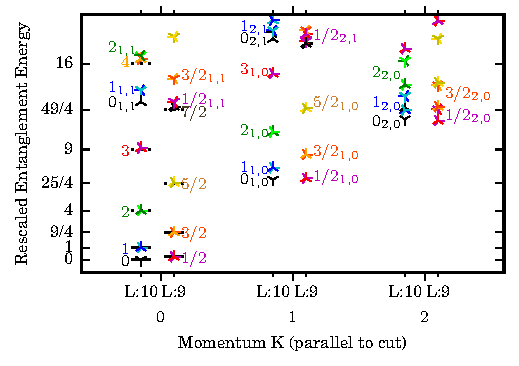
\includegraphics[width=\columnwidth]{EEIdentify.pdf}
		\vskip-3ex
	\caption{The identification of the primary states $\ket{\pm e, m=0}$ and the level $n, \bar{n}$
	descendants in the spectrum of the soft-core boson entanglement Hamiltonian. The states are labeled
	$e_{n, \bar{n}}$. The zero and scale of the numerical spectrum are set by matching the lowest two
	states. The energies and charges of the primaries with charges $2, 5/2, ... 4$ appear at the predicted
	spots.  The best estimate for the Luttinger parameter from this spectrum is $\kappa \approx 1.6$,
	taken from the energy of the $0_{1, 0}$ state. }
	\label{fig:EEIdentify}
\end{figure}


However, the states with non-zero winding number $m$, such as $\ket{0, \pm 1}$, do not appear at
the energy and momentum predicted by the above formula. Instead, the primary states $\ket{e, m=\pm
1}$ can be found centered around momentum $K=\pi$. The identification of these states in the spectrum
is shown in Figure~\ref{fig:EEIdentifyPi}. Although the larger $m$ states are too high in energy 
to be reliably distinguished at this system size, a natural conjecture is that all primaries with 
odd $m$ will appear around momentum $\pi$.

\begin{figure}[htbc]
	\centering
	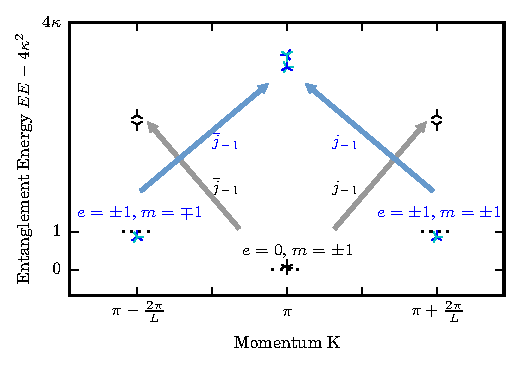
\includegraphics[width=\columnwidth]{EEIdentifyPi.pdf}
		\vskip-3ex
	\caption{The identification of primary states $\ket{e, m=\pm1}$ and first descendants in the low energy part of the spectrum near momentum $\pi$. Unlike the $m=0$ states shown in Figure~\ref{fig:EEIdentify}, these primary states have shifted momentum $K = \pi + em (2\pi/L)$ and an extra double degeneracy due to the two values of $m=\pm1$. Using the estimate $\kappa \approx 1.6$ from Figure~\ref{fig:EEIdentify}, the predicted value of the entanglement energy for the $\ket{e=0, m=\pm1}$ states is $4\kappa^2$, which has been marked in the plot. The agreement is very good. \brayden{j, jbar switched on arrows, also maybe just simplify this}}
	\label{fig:EEIdentifyPi}
\end{figure}

Given the PEPS representation, we can express the entanglement Hamiltonian $H_L$ for
the left semi-infinite cylinder, defined via $\rho_L = \exp(-H_L)$, as a Hamiltonian acting on the auxiliary
degrees of freedom of the PEPS crossing the cut, which we have denoted as $|\sigma_1,\ldots,\sigma_W)$.
We expect this Hamiltonian to encode the universal properties of the edge CFT, which should be invariant
under local gauge choices in the PEPS. Its ground state is (up to normalization) given as
\begin{equation}
|\Psi_0) = \sum_{\sigma_1,\ldots,\sigma_W} \langle \Psi^{(\sigma_1,\ldots,\sigma_W)}|\Psi_L^{(0)}\rangle |\sigma_1,\ldots,\sigma_W).
\end{equation}
In Fig.~\ref{fig:EdgeGS_EE}, we show the bipartite von Neumann entanglement entropy of this state for a cut
into $l$ and $W-l$ sites, which confirms the central charge of the edge CFT.

%Since we have the local basis $\ket{\psi_L^{(\sigma_1, \ldots, \sigma_W)}}$ of $2^W$ states with charges matching those of a spin $\frac12$ chain of length $W$, it is tempting to think of the entanglement Hamiltonian as a critical theory on a spin $\frac12$ chain of length $W$. This analogy cannot be exact, because this basis of states is not orthonormal. Still, we find that the coefficients $u^{(0)}_{\{\sigma_i\}}$ of this state in the local basis
%$$\ket{\psi_L^{(0)}} = \sum\limits_{\{\sigma_i\}} u^{(0)}_{(\sigma_1, \ldots, \sigma_W)} \ket{\psi_L^{(\sigma_1, \ldots, \sigma_W)}}$$
%have entanglement properties similar to a critical 1D ground state wavefunction with central charge $c=1$. This result is shown in Fig.~\ref{fig:EdgeGS_EE}.

\begin{figure}[htbc]
	\centering
	\includegraphics[width=\columnwidth]{{EdgeGS_EntanglementEntropy.pdf}}
	\caption{Entanglement entropy within the entanglement ground state
of the soft-core boson state on $10$ sites. For comparison, the
Cardy-Calabrese formula $S(x) = c/3 \log \sin( \pi x/L) + const.$ is
shown with $c=\frac{1}{2}, 1,$ and $2$, with the $const.$ fixed by
matching the maximum of the entanglement entropy data. $c=1$ is a good
fit.}
	\label{fig:EdgeGS_EE}
\end{figure}